Bright sources present a potential stress case for large-format focal plane electronics, motivating dedicated on-sky tests during LSSTCam commissioning. Extremely bright stars can, in principle, induce elevated charge levels that when read out can induce a safety response in the associated REB to power off CCDs as the readout current increases. Monitoring telemetry in response to high-flux signals is therefore a useful diagnostic for identifying unintended behavior between optical illumination and detector electronics.

The analysis presented here is based on the notebook \href{https://github.com/lsst-sitcom/LSSTCam-OnSkyTests/blob/main/notebooks/brightStarTests.ipynb}{\texttt{brightStarTests.ipynb}} in the LSSTCam On-Sky Tests repository and focuses specifically on REB bias currents measured during and around bright-star exposures.

\subsubsection{Test Description}

The dataset consists of a sequence of on-sky exposures targeting bright stars with approximate apparent magnitudes of 0 (Alpha Centauri), 1 (tet Cen), and 2 (* gam Crv). These exposures were obtained by placing the stars on the central detector of specific REBs in the LSSTCam focal plane.

The following rafts and REBs were included in the study:
\begin{itemize}
    \item R01/Reb1
    \item R01/Reb2
    \item R02/Reb1
    \item R02/Reb2
\end{itemize}

These REBs were selected based the results of Run 7, focusing on REBs that had tripped in response to high-flux exposures during the course of testing  \citep{SITCOMTN-148}.

Exposure numbers were used to retrieve precise timestamps from the exposure metadata, and fixed time offsets were applied to define consistent pre- and post-exposure windows.

\subsubsection{Data}

Telemetry was retrieved from the Engineering and Facility Database using the SAL topic \texttt{lsst.sal.MTCamera.rebpower\_Reb}. From this topic, fields associated with pre-switch bias currents (\texttt{hvbias\_IbefSwch}) were selected for analysis. 

For each exposure, telemetry was queried over a time range extending one minute before and after the nominal exposure start time. This approach allows transient effects to be distinguished from nominal baseline behavior.

\subsubsection{Method}

For each exposure and REB, time-series plots of the selected bias currents were generated. The analysis focused on identifying:
\begin{itemize}
    \item Sudden current excursions coincident with bright star illumination.
    \item Sustained offsets relative to pre-exposure baselines.
    \item Differences in behavior between rafts or stellar magnitudes.
\end{itemize}

Exposure timing was used as a visual reference for identifying correlated behavior. No filtering or smoothing beyond the native telemetry cadence was applied.

\subsubsection{Results}

Across all examined exposures, stellar magnitudes, and REBs, the bias-current telemetry remains within the acceptable safety limit of 120\,mA. No current excursions above $97\text{mA}$ are observed. No discontinuities, or systematic trends were observed during or after the bright-star exposures. This holds across the entire set of rafts, indicating that the response is uniform across the focal plane.

\begin{figure}
    \centering
    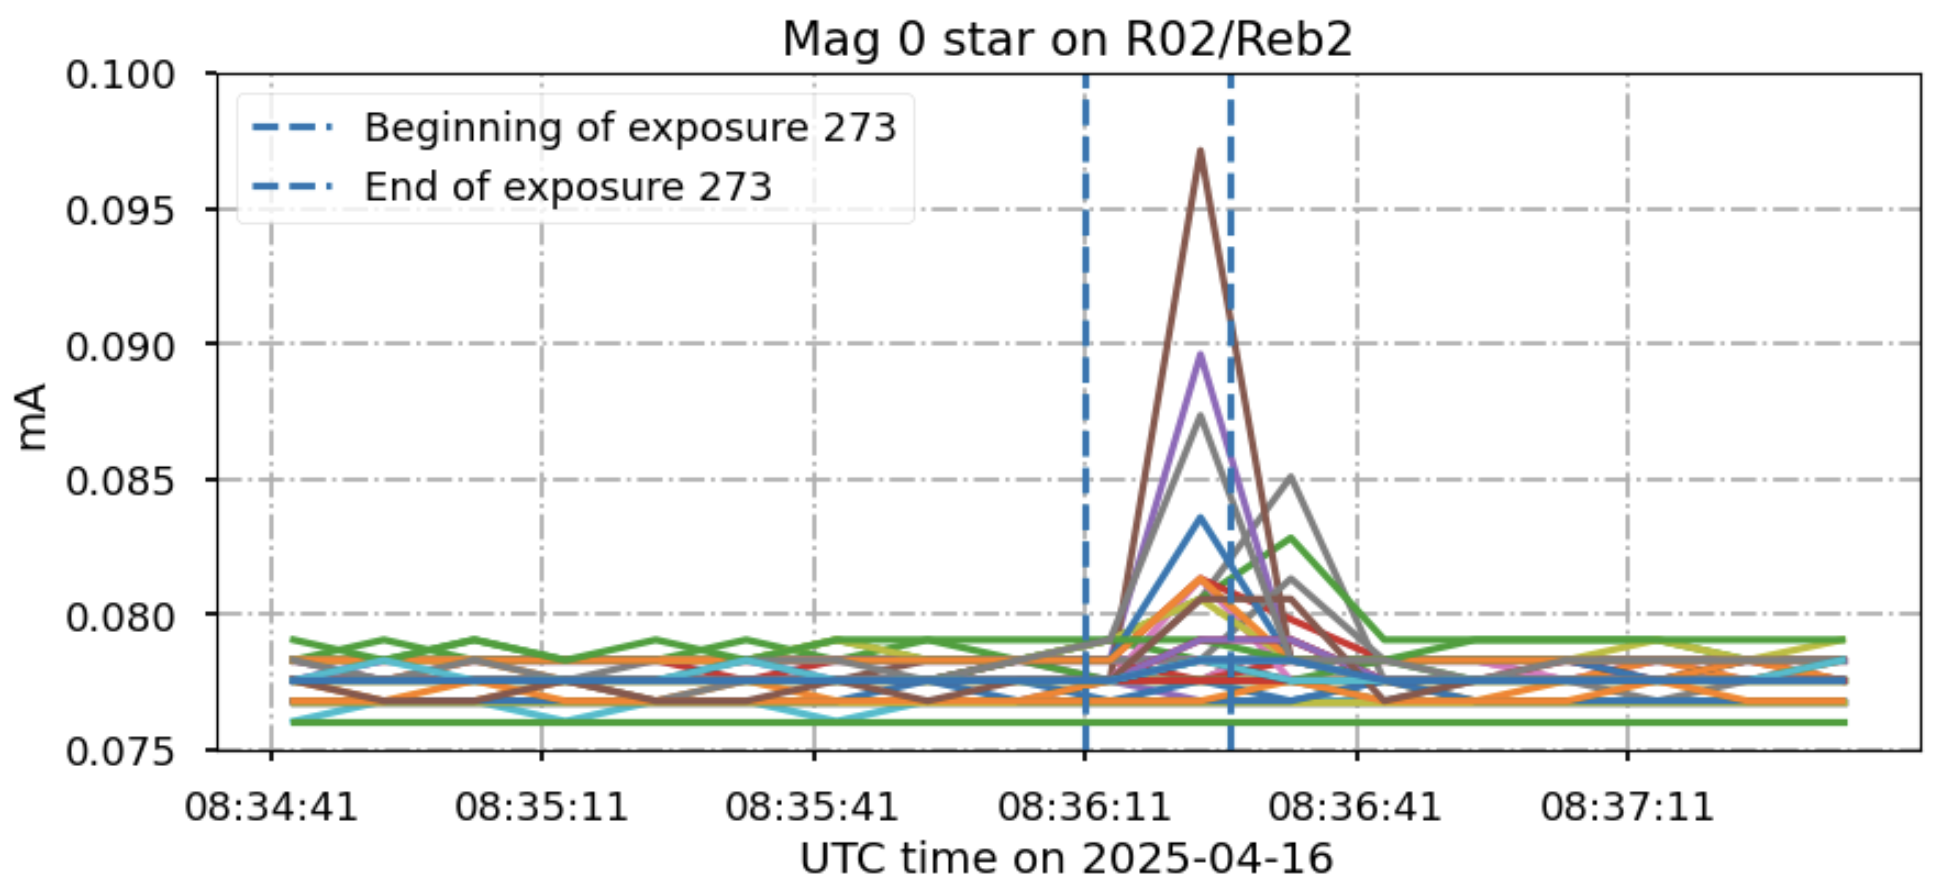
\includegraphics[width=1\linewidth]{onskyperformance//figures/bright_star_exp.png}
    \caption{The largest current excursion observed during the bright star test. The vertical dashed lines indicate the start and end of the exposure. The solid lines indicate the measured current on each REB.}
    \label{fig:bright_star_current}
\end{figure}

Telemetry inspection shows that any small-scale fluctuations in the currents are comparable to those seen outside of the exposure windows and are consistent with nominal electronic noise rather than illumination-induced effects.

\subsubsection{Conclusion}

These results indicate that bright star illumination at the tested magnitudes does not induce measurable perturbations in REB bias currents. This provides confidence that LSSTCam electronics operate stably even in the presence of bright optical sources up to magnitude 0, and that such sources do not pose a risk to detector safety.

In summary, no evidence is found for anomalous electrical behavior correlated with bright-star exposures. These results verify the robustness of LSSTCam electronics under high-flux observing conditions and validate current operational assumptions for bright-source observations.
